\documentclass[article]{uom-coursework}

\usepackage{blindtext}
\usepackage[showframe]{geometry}
\usepackage{float}
\usepackage[backend=biber]{biblatex}
\addbibresource{dsa.bib}

\counterwithout{section}{chapter}

% Biblography
% \addbibresource{dsa.bib}

\title{Data Structures and\\Algorithms 2}
\tagline{Coursework}
\author{Juan Scerri}
\authorid{1234567A}
\courseworkname{Some Degree}
\doctype{coursework}
\courseworkdate{\monthyeardate\today}
\subjectcode{ICS2210}


\begin{document}

%----------------------------------
%	Front Matter
%----------------------------------

\pagestyle{umpage}

\frontmatter

\maketitle % Print the title page

\tableofcontents % Print the table of contents

\clearpage

\lstlistoflistings

\clearpage

\mainmatter

% \chapter{Report}

\chapter*{Report}
\label{chap:report}
\addcontentsline{toc}{chapter}{\nameref{chap:report}}

\section{Language}

The programming language used for this coursework is Python 3.
The main reason for this choice is the speed of development.

\section{Knuth Shuffling}

\lstinputlisting[caption={A function implementing Knuth shuffling.},language=Python,firstline=8,lastline=13]{../ics2210/knuth_shuffling.py}

Knuth shuffling, also known as Fisher--Yates shuffling, is an
algorithm used for generating permutations of the elements of a
given array.

The implementation follows the pseudocode described here in
\textcite{wikifisheryates}.

\section{Binary Search Tree}

First a Binary Search Tree (BST) was implemented. This is
because the basic structure of a BST underlies both
Adelson-Velsky-Landis (AVL) and Red-Black trees, helping reduce
code duplication.

The file \texttt{untyped\_tree.py} contains two of our base
building blocks. In particular these are \texttt{Node} and
\texttt{Tree}. As described the \texttt{Tree} class is a BST
with the main method being \texttt{insert()}. This is a basic
BST insert. Note however that a number of methods associated
with the Node class are being used.

Additionally, when creating a tree one can enable statistics to
keep track of the number of steps required for insertion to
complete.

Other methods required for collecting certain statistics
include: \texttt{calc\_height()} and \texttt{calc\_leaves()}.
They are quite self-explanatory, one is used to calculate the
height of the tree whilst the other is meant to calculate the
number of leaves the tree has.

The only issue with these methods is that they are recursive.
However, since the trees under consideration will be balanced
and are limited to 6000 nodes, they are well within the
recursion limit of the language. However, this is of course not
ideal and iterative approaches should be preferred.

The \texttt{draw()} method as its name implies allows the trees
to be drawn and printed to the terminal. This method was
invaluable during development to ensure correctness of
algorithms by checking for parity with other implementations,
specifically those found at
\url{https://www.cs.usfca.edu/~galles/visualization/}.

If you wish to test the implementations for yourself please
either use \texttt{python} or \texttt{ipython}. Additionally,
please ensure that you are in the root directory of the project.
Then follow the commands used in Figure \ref{fig:ipythonavl} and
Figure \ref{fig:ipythonskip}.


\begin{figure}[H]
\centering
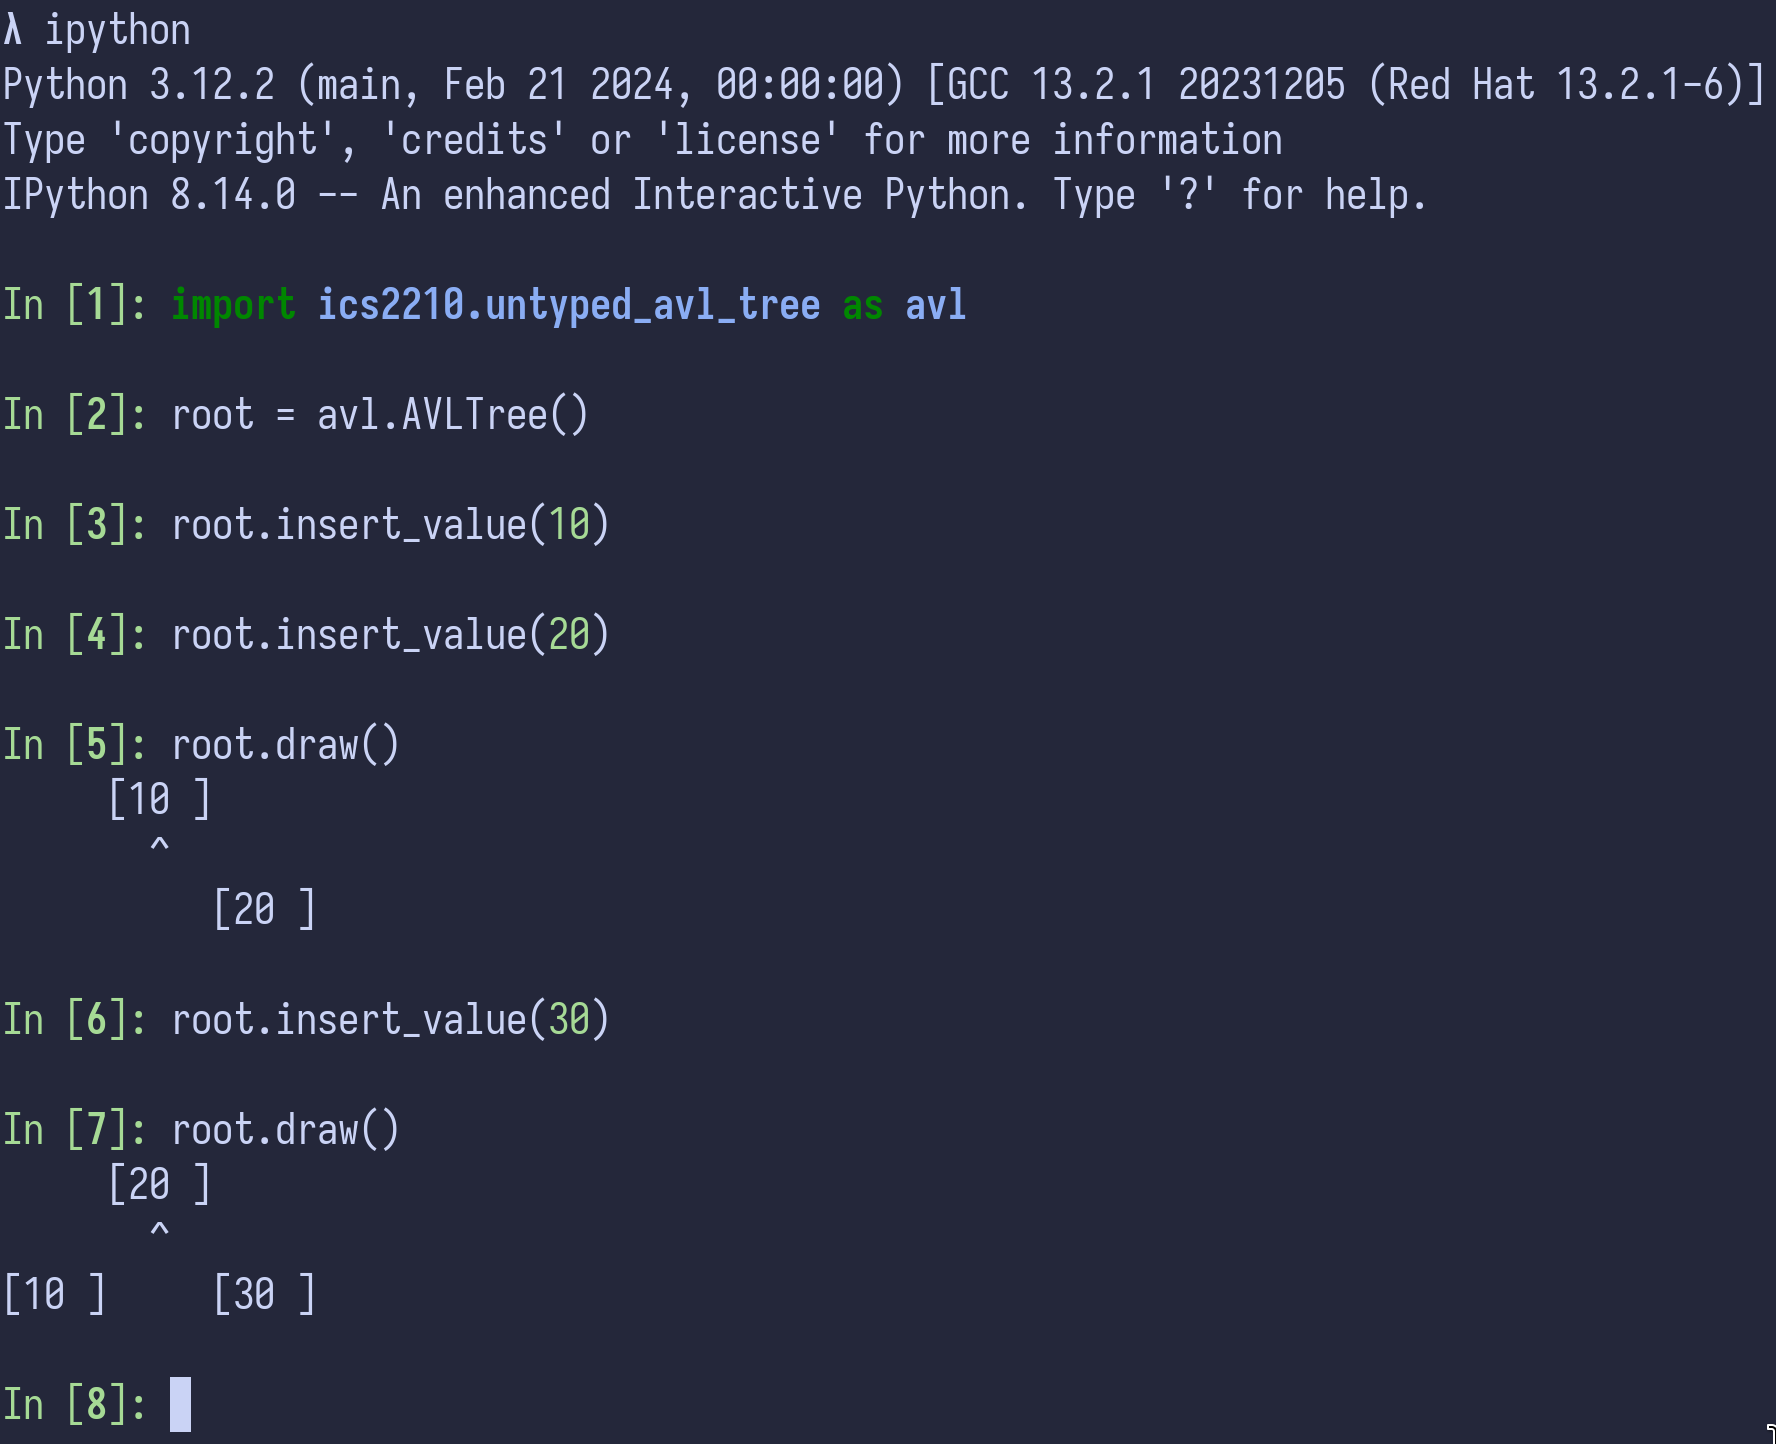
\includegraphics[width=\linewidth]{using-ipython-avltree.png}
\caption{Using an \texttt{AVLTree} (similar
interface for an \texttt{RBTree}).}
\label{fig:ipythonavl}
\end{figure}

\begin{figure}[H]
\centering
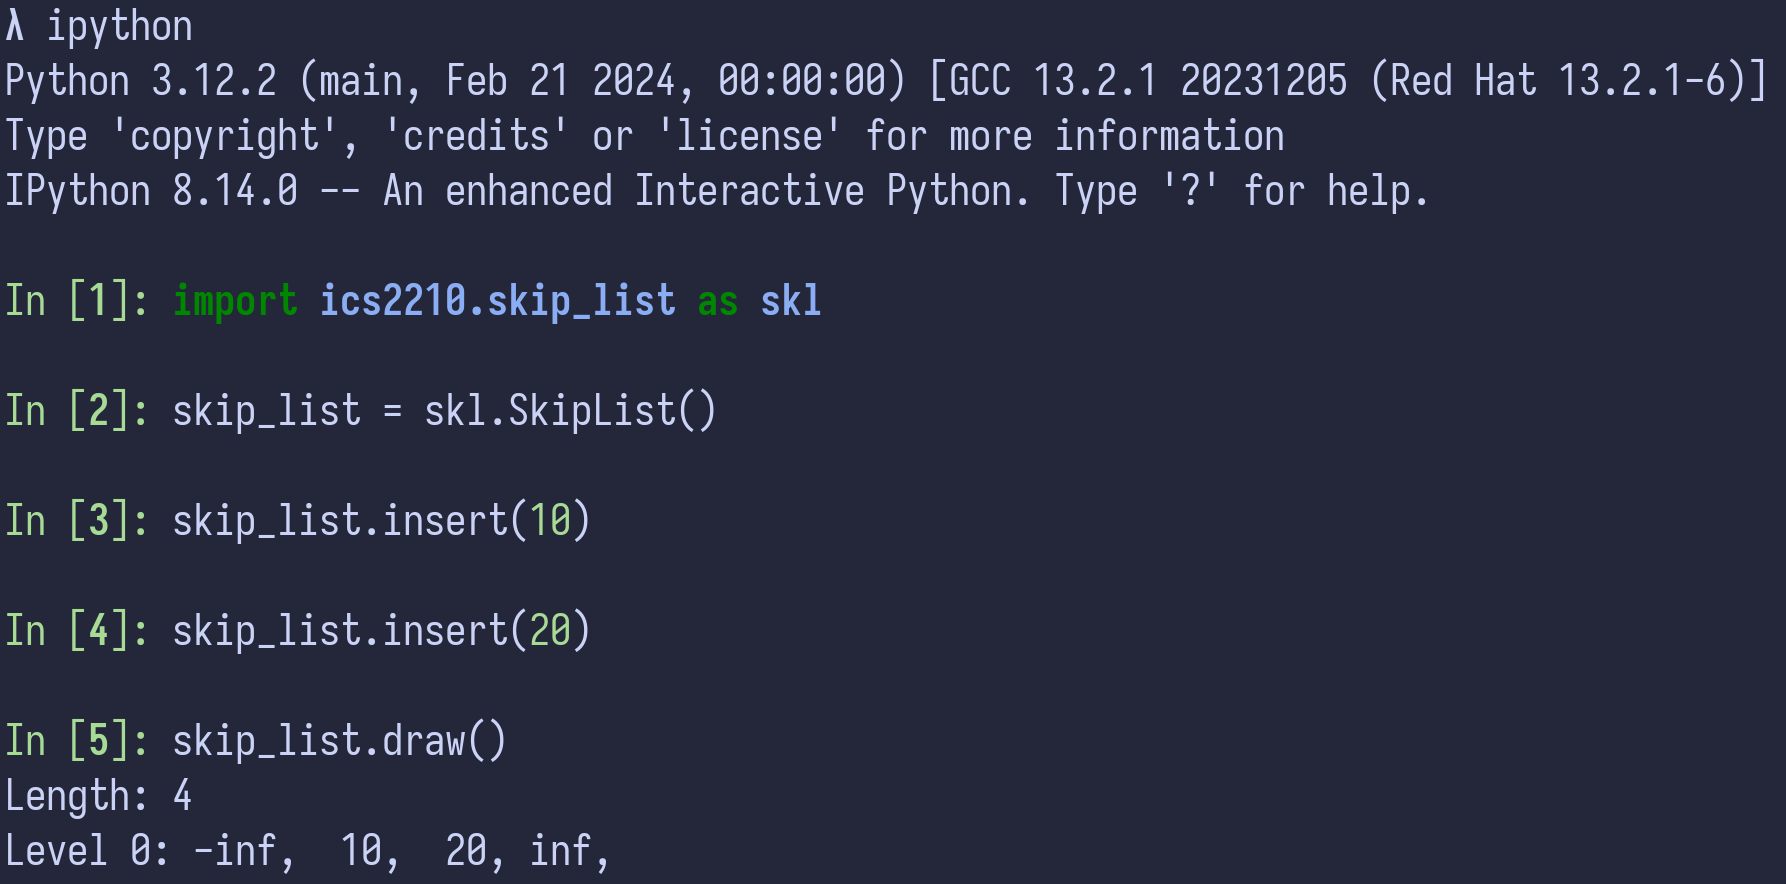
\includegraphics[width=\linewidth]{using-ipython-skiplist.png}
\caption{Using a \texttt{SkipList}.}
\label{fig:ipythonskip}
\end{figure}

Additionally, these classes have a baked in example which can be
run to test their behaviour (see Figure \ref{fig:example}).

\begin{figure}[H]
\centering
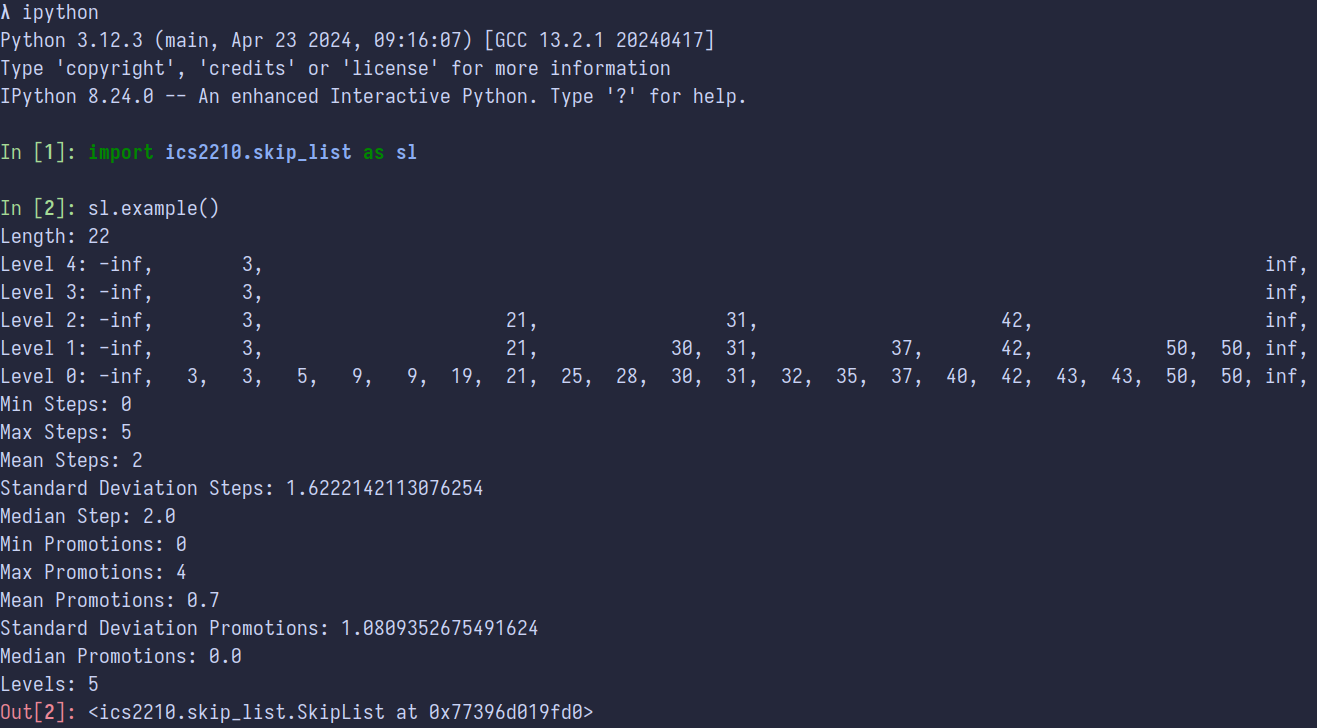
\includegraphics[width=\linewidth]{ipython-skiplist-example.png}
\caption{Using the builtin \texttt{SkipList} example (the
\texttt{AVLTree} and \texttt{RBTree} classes both also have a
builtin example).}
\label{fig:example}
\end{figure}

The \texttt{Node} class is a bit more complicated. It is not
simply a pure node, it contains a variety of methods which help
facilitate readable code within the encompassing data
structures, specifically the \texttt{AVLTree} and
\texttt{RBTree} classes.

The following methods are of particular interest:
\texttt{rotate()}, \texttt{can\_step()}, \texttt{value\_dir()}
and \texttt{dir()}. The other present method are fairly simple
and straight forward.

The \texttt{can\_step()} method returns a boolean allowing
indicating to the callee whether or not a node has a child in
the specified direction.

The \texttt{value\_dir()} accepts a value which can be compared
with the value present in the node. Then depending on whether
the value is greater than or less than the value in the node a
direction is provided. In particular, if its is less than, the
\texttt{LEFT} direction will returned and if it is greater than
(or equal to) the \texttt{RIGHT} direction is returned.

\texttt{dir()} is used to check whether an other node is on the
left or right of the current node.

NOTE: this method is unsafe in the
sense that if a other node is provided and it is not a child the
self node then it will be classified as being on the right of
the node which is of course
incorrect.


\texttt{rotate()} finally the rotate
method is a generalized ll or rr
rotation method. Note that lr and
rl can be achieved by using combinations
of ll and rr.

Additionally, this rotate method has been heavily
inspired by the rotate method used on
wikipedia for the implementation
of red-black trees.


\section{AVL Trees}

AVL Trees where implemented my first inhereting
from the base classes described above.
The \texttt{left\_height} and \texttt{right\_height}
fields where added as they are required for the
algorithm to work. Additionally, the
\texttt{height\_diff()} allows us to calculate
the difference in height for a specified AVLNode.
Additionally, the \texttt{update\_heights()} method
allows us to recompute the height of current AVLNode.
This is important because the relevant
node need to have their heights update after every
rotation.

\begin{lstlisting}[caption={The main insert function for AVL Trees},language=Python]
def insert(self, node):
    self.root = self.fix(super().insert(node))
\end{lstlisting}

The \texttt{fix()} method is the method which
rebalances the tree after an insertion. It mostly
an intuitive implementation of the algorithms
as they would be described on a piece of paper.

In particular we start from the node that has just been inserted
and check that each node during a traversal upto the root that
each node within said path is balanced. If not one of the
rebalancing algorithms ll, lr, rr or rl is employed. Note that
at the end the root is returned. This is critical because the
root of the tree can change due to rotations.

The code is of course sprinkled with bits and piece
which keep track of the necessary statistics.

In particular, use of the fact that if statements
in python do not create a scope of there own is being
used.

\section{Red-Black Trees}

Similarly, as discussed in the previous section,
The RBNode and RBTree classes inherit from
their respective bases classes. The RBNode
class has two additional methods,
\texttt{sibling\_is\_red()} and \texttt{get\_sibling()}.
Note that in this case both methods assume that the current
node has a parent and therefore it is guaranteed to have
a sibling (if the left/right node is \texttt{None} it is
still considered to be a node and it is treated as a black).

The RBTree class similarly to the AVLTree class has a
\texttt{fix()} method. The \texttt{fix()} method again starts at
the inserted node and traverse up to the root, and at each step
if a necessary change is required. Note that the \texttt{fix()}
for an RBTree does not need to traverse up the whole tree to the
root.

Again similarly the same mechanism for collecting statistics is
used.

\section{Skip Lists}

Before implementing a Skip List an
extended integer class was defined. In particular
This set of objects instantiated by the extended
integer class is set of all integers and the
objects $-\infty$ and $\infty$. Of course
the most natural property these objects, which
are called ``infinity'', have is the
following:

$$\forall z \in \mathbb{Z} \cup \{-\infty, \infty\}, -\infty \leq z \leq \infty$$

The main reason for the inclusion of this type is to facilitate
a more natural implementation of Skip Lists. In particular this
helps avoid issues with not having a top-most left element.

\begin{figure}[H]
\centering
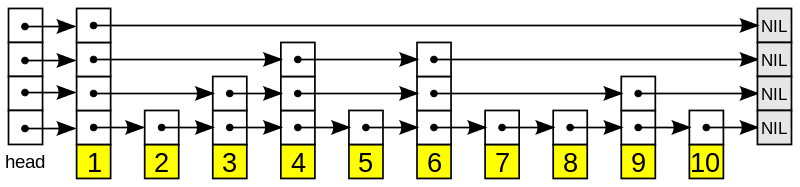
\includegraphics[width=\linewidth]{wikipedia-skip-list.png}
\caption{An graphical depiction of a Skip List (source: \url{https://en.wikipedia.org/wiki/File:Skip_list.svg}).}
\label{fig:test9}
\end{figure}

The above figure was a great inspiration with regards
to the implenetation details of the Skip List.
Each element in the skip list is called a SkipNode.
And a skip node is a value and a list/array of pointers.

It has two classmethods which generate the head and tail nodes.
Along with an \texttt{add\_level()} method which allows for the
addition of a element in the list of forward pionters.
Finally, the \texttt{add()} method allows the addition
of an element at a specific level.

Finally, the skip list itself keeps track of the head and tail
of the list along, with the height and length. Additionally,
if enabled the specified statistics will also be collected.


Again \texttt{insert()} is the main method for the SkipList
class. In particular it traverses the skip list keeping
track of all the nodes which contain the largest
value less than or equal to the value we want to insert.
These values are kept in a stack as the algorithm traverses
down the list.

Keeping track of these nodes is important for the second phare
of the insertion alogrithm. Since after inserting in the lowest
level, a node can be promoted a random number of times, in the
case where the promotion does not exceed the height of the Skip
list, the new node needs to be linked with one of the nodes the
algorithm kept a reference to in the stack. Ensuring that the
ordering of a skip list is not violated. 

\section{The \texttt{procedure.py} File}

This file which contains the procedure of steps as described
within the coursework. The requirements for running the file are
present within the \texttt{README.md} file. To reiterate
please ensure that at \texttt{python} version \texttt{3.11.8}
is installed. Other version of \texttt{python} have not
been \textbf{tested}.

Since the \texttt{procedure.py} has been marked by a
\texttt{\#!/usr/bin/env python3} and made executable it can be
run using \texttt{./procedure.py} from the root directory of the
project. Additionally if that does not work it can be run with
\texttt{python3 procedure.py} again from the root directory.

\section{Discussion}

Running \texttt{./procedure.py} yields the following
result:

\begin{lstlisting}[]
[juan@arch] dsa2-coursework
λ ./procedure.py 
--- Inserting the first 5000 integers! ---

AVL Tree Stats:
Min Steps: 0
Max Steps: 14
Mean Steps: 10.076415283056612
Variance Steps: 2.8112863869292464
Median Step: 10
Min Rotations: 0
Max Rotations: 1
Mean Rotations: 0.4612
Variance Rotations: 0.24854426885377076
Median Rotations: 0.0
Height: 14
Leaves: 2153

RB Tree Stats:
Min Steps: 0
Max Steps: 14
Mean Steps: 10.098219643928786
Variance Steps: 2.9101188785176
Median Step: 10
Min Rotations: 0
Max Rotations: 1
Mean Rotations: 0.3874774954990998
Variance Rotations: 0.23738617271273382
Median Rotations: 0
Height: 14
Leaves: 2169

Skip List Stats:
Min Steps: 0
Max Steps: 33
Mean Steps: 11.3456
Variance Steps: 31.08917847569514
Median Step: 11.0
Min Promotions: 0
Max Promotions: 12
Mean Promotions: 0.9664
Variance Promotions: 1.7932296859371875
Median Promotions: 1.0
Levels: 13

--- Inserting the other 1000 integers! ---

AVL Tree Stats:
Min Steps: 0
Max Steps: 14
Mean Steps: 10.394065677612936
Variance Steps: 3.0044062584399835
Median Step: 11
Min Rotations: 0
Max Rotations: 1
Mean Rotations: 0.468
Variance Rotations: 0.24901750291715286
Median Rotations: 0.0
Height: 14
Leaves: 2585

RB Tree Stats:
Min Steps: 0
Max Steps: 15
Mean Steps: 10.579429904984163
Variance Steps: 3.7438982411262165
Median Step: 11
Min Rotations: 0
Max Rotations: 1
Mean Rotations: 0.39323220536756126
Variance Rotations: 0.2386404180623413
Median Rotations: 0
Height: 15
Leaves: 2597

Skip List Stats:
Min Steps: 0
Max Steps: 33
Mean Steps: 11.29
Variance Steps: 28.28828138023004
Median Step: 11.0
Min Promotions: 0
Max Promotions: 12
Mean Promotions: 0.9691666666666666
Variance Promotions: 1.7898476134911374
Median Promotions: 1.0
Levels: 13
\end{lstlisting}

In light of the above statistics first a number of
a few seemingly anomalies will be discussed then
the data structures will be compared.

\subsection{The Oneness of Balanced Trees}

A particularly interesting observation is the strange
outcome that after 6000 insertions both AVL trees and
Red-Black trees only ever use at most one rotation
to rebalance. This is by no means an oddity.
As mentioned by the Wikipedia article
on Red-Black trees at \url{https://en.wikipedia.org/wiki/Red-black_tree#Notes_to_the_insert_diagrams}, specifically,
the last bullet point. Insertion of Red-Black trees
can incur at most 2 rotations. In our case a single
rotation is being counted since as specified
by the report although lr and rl are composed of
two rotations they are treated as one as per the
coursework specification.

\subsection{Comparing AVL Trees and Red-Black Trees}

things I would like to point out

AVL trees and Red-Black trees are deterministic
The efficiency of Skip-List although indentical
to AVL and Red-Black trees. It is only so in a probabilistic
sense. This means that the effectiveness of Skip-Lists
is dependent on whether the source of
randomness is truly random or not. Since the pseudo-random
number generate will introduce a bias.

Now depending on the environment in which a Skip List will
determine its effectiveness. In particular although
it is not clear from my implementation the size of
a Skip List in terms of the number of instructions
required to implement it is significantly smaller than
that of an AVL or Red-Black tree. Hence, it might 
be useful to implement such algorithm if
an efficient data structure is required in a specific
application where the space constraints of the programmable
device are a real consideration. This of course will entail
researching and benchmarking the performance of the
Skip lists with a number of synthetic data sets that it might
experience in the wild and whether the random number generation
introduces any bias.

It is also crucial to point out that all three different
implementations are not very cache friendly. They all use
pointers and systems notoriously have a hard time increasing the
cache-hit rate of data structures which are not contiguous. Of
course skip lists and the trees are fundamentally different
types and they have different cache characteristics but none
will ever be as good as a fixed size array for example.

A slight note on thread-safety. As mentioned in this post on
StackOverflow \url{https://stackoverflow.com/questions/256511}.
Locking locality can be a consideration. In particular a skip
list can be easily augmented to support multithreaded insertion
This is because for every insertion a skip list only needs to
lock the two neighbouring skip nodes. However, as mentioned in
the above post there do seem to exit lock-free Red-Black tree
implementations.

It is also important to mention that the tree-based algorithms
are guaranteed to give the performance they advertise in regards
to worst-case complexity, that being $O(\log n)$ for all cases
of search, insert and delete for both AVL and RB trees. In the
context of Skip Lists there is not such guarantee.

Additionally, as indicated by the standard deviation in the
number of steps required to reach the adequate position in a
Skip List varies more significantly. This indicates a more
uniform access time in AVL or RB trees.

Hence, in the context of a normal general purpose
computer that has enough memory to load all the instruction
for an AVL tree or a RB tree. An AVL tree and a
RB tree should be used.

\subsection{AVL Trees vs.\ Red-Black Trees}

Now that trees vs.\ skip lists has been discussed, AVL trees
vs.\ Red-Black trees will be discussed.

\begin{figure}[H]
\centering
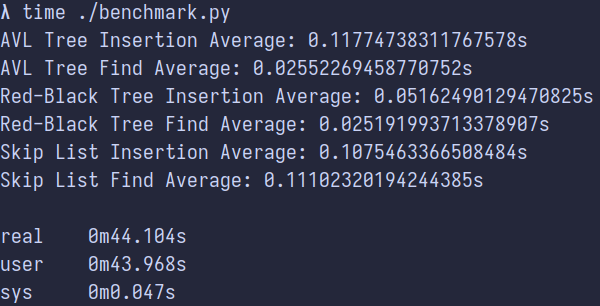
\includegraphics[width=\linewidth]{benchmark.png}
\caption{An insertion benchmark calculating the average amount of time
in seconds it would take to insert 10000 elements into each
data structure on a single-thread as fast as possible.}
\label{fig:test9}
\end{figure}

\begin{figure}[H]
\centering
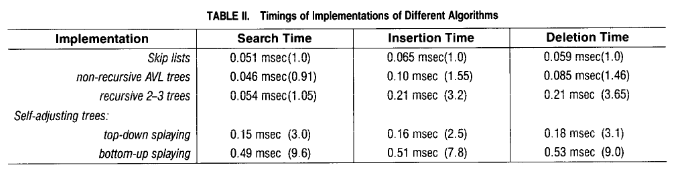
\includegraphics[width=\linewidth]{table2-pugh.png}
\caption{A figure of Table 2, as presented in \textcite{pugh90}.}
\label{fig:test9}
\end{figure}


In particular in \textcite{pugh90}, specifically table 2,
the author claims that AVL trees have an insertion time
twice as slow as insertion in Skip Lists. Of course
as can be seen in the above benchmark of the current
the implementation this is not the case. In fact
it is on equal footing with AVL trees. Hence,
in a choice over whether to use AVL trees or Skip Lists
in a normal environment AVL trees would be my pick.

However, even though AVL trees are technically always a bit
shorter than Red-Black trees which have at height at most $2
\log (n + 1)$ where $n$ is the number of vertices, they are
faster at insertion whilst AVL trees are faster at searching.

Why is this the case? In particular as we discussed AVL trees
are guaranteed to never be as long as a Red-Black tree. This
means that searching in an AVL will be faster. However,
when inserting in an AVL an implementation will have to traverse
the whole height of the tree twice. Why? When inserting
we are guaranteed to traverse the whole tree to reach a leaf
vertex so that is $\log n$ operations. But then
the algorithm needs to traverse back up to the root
this is because the local information available to the algorithm
at any specific is not enough information to guarantee
that the rest of the tree is balanced. Hence,
insertion is always a $O(2 \log n)$ operation in an AVL tree.

In a Red-Black tree the algorithm performs at most $2 \log (n + 1)$ operations
to go down to the leaf nodes. However, the algorithm can terminate
in the first instance it reaches a black node since it guarantees
the balance constraints of the whole tree. Now as we can see from the
statistics on average a Red-Black tree actually often has the same height
as an AVL tree which means it has the added benefit of shorter
insert times along with an almost equivalent search time.

This is reflected in our benchmark. In fact, Red-Black trees are
more than twice as fast as AVL trees when inserting and as fast as
AVL trees when searching.

Hence between a AVL tree and a Red-Black tree. 
Our testing mostly concludes that a Red-Black tree should
be the default choice if we wish for a data structure
which exhibits the general an $O(\log n)$ complexity
for all three main operations search, insert and delete.

However, in the eventually that a harder restriction on search speed is required
AVL trees should be used since they are guaranteed to shorter
than Red-Black trees.

\printbibliography

\end{document}
